\chapter{A Lattice-Boltzmann model for acoustics}

Given an ideal particle system described by a number density function $f(\vec x, \vec v_i, t)$ defined as the probability to find a particle at the position $\vec x$ with a given velocity $\vec v_i$ at the instant of time $t$, the Lattice-Boltzmann equation as a discretized form of the Boltzmann transport equation is written, in general, as follows
\begin{equation}\label{eq:LBE}
    f_i(\vec x + \vec v_i \delta t, t + \delta t) = f_i(\vec x, t) + \Omega_i(\vec x, t)    
\end{equation}
Where $\Omega_i(\vec x,t)$ is the collision operator. If the Bhatnagar-Gross-Krook (BGK)
\begin{equation}\label{eq:BGK}
    \Omega_i(\vec x,t) = -\delta t\frac{f_i(\vec x, t) - f^{\text{eq}}(\vec x, t)}{\tau}
\end{equation}
is used, with $\tau$ the relaxation time, then the equation \ref{eq:LBE} becomes
\begin{equation}\label{eq:LBE_BGK}
    f_i(\vec x + \vec v_i \delta t, t + \delta t) - f_i(\vec x, t) = -\delta t\frac{f_i - f^{\text{eq}}}{\tau}
\end{equation}
where $f^{\text{eq}}$ is defined as the equilibrium distribution function.

This distribution function \textbf{is relaxed to the one at equilibrium} such that the following macroscopic moments are obtained:
\begin{subequations}\label{eqs:moments}
\begin{equation}
    \Pi^{\text{eq}} = \sum_i f_i^{\text{eq}} \label{eq:moment0}
\end{equation}
\begin{equation}
    \Pi^{\text{eq}}_{\alpha} = \sum_i v_{i\alpha}f_i^{\text{eq}}\label{eq:moment1}
\end{equation}
\begin{equation}
    \Pi^{\text{eq}}_{\alpha\beta} = \sum_i v_{i\alpha}v_{i\beta}f_i^{\text{eq}}\label{eq:moment2}
\end{equation}
\begin{equation}
    \Pi^{\text{eq}}_{\alpha\beta\gamma} = \sum_i v_{i\alpha}v_{i\beta}v_{i\gamma}f_i^{\text{eq}}\label{eq:moment3}
\end{equation}
\end{subequations}
The definition of these moments will be covered later, the equilibrium distribution function must be chosen such that summing over $i$ multiplied by the corresponding order of $\vec v_i$ the desired moments are gotten.

As the space and time are discretized, the velocities set $\{\vec v_i\}$ are discretized as well in a defined set in general defined as D$d$Q$q$ where $d$ is the dimension of the lattice and $q$ is the amount of vectors existing per cell. Some examples are D3Q19 or D2Q9. 
% \begin{columns}[c]
% \column{.5\textwidth}
% \begin{figure}
% \centering
% 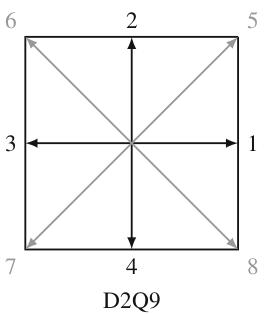
\includegraphics[width=.5\textwidth]{D2Q9.png}
% \caption{\small D2Q9 lattice set.}
% \end{figure}
% \column{.5\textwidth}
% \begin{figure}
% \centering
% 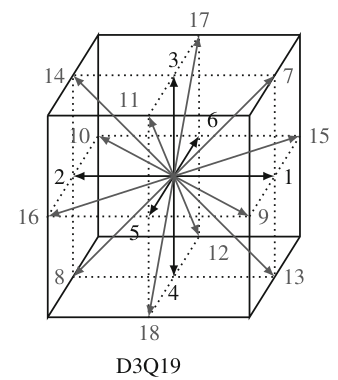
\includegraphics[width=0.6\textwidth]{D3Q19.png}
% \caption{\small D3Q19 lattice set.}
% \end{figure}
% \end{columns}

For each velocities set there is a set of weights constants $\{\omega_i\}$ associated for each velocity, so that now we define a set of velocities and weights $\{\vec v_i,\omega_i\}$ which satisfies the following conditions:
\begin{subequations}\label{eqs:sums_vw}
\begin{equation}\label{eq:sum_wi}
    \sum_i \omega_i = 1
\end{equation}
\begin{equation}\label{eq:sum_viwi}
    \sum_i v_{i\alpha}\omega_i = 0
\end{equation}
\begin{equation}\label{eq:sum_viviwi}
    \sum_i v_{i\alpha}v_{i\beta}\omega_i = c_s^2\delta_{\alpha\beta}
\end{equation}
\begin{equation}\label{eq:sum_viviviwi}
    \sum_i v_{i\alpha}v_{i\beta}v_{i\gamma}\omega_i = 0
\end{equation}
\begin{equation}\label{eq:sum_viviviviwi}
    \sum_i v_{i\alpha}v_{i\beta}v_{i\gamma}v_{i\mu}\omega_i = c_s^4(\delta_{\alpha\beta}\delta_{\gamma\mu} + \delta_{\alpha\gamma}\delta_{\beta\mu} + \delta_{\alpha\mu}\delta_{\beta\gamma})
\end{equation}
\end{subequations}
Where $c_s^2$ is \textbf{for now a constant}.

In order to gather the PDE satisfied by the macroscopic moments defined at \ref{eqs:moments} we need to develop a \textbf{Chapman-Enskog analysis}. If the continuous transport Boltzmann equation is written as 
\begin{equation}\label{eq:C_LBE}
    \bigg(\partial_{t} + v_{i\alpha}\partial_\alpha\bigg)f_i = -\frac{\delta t}{\tau}(f_i - f^{\text{eq}})
\end{equation}
defining $\partial_t = \partial/\partial t$ and $\partial_\alpha = \partial/\partial x_\alpha$, a Taylor expansion is done in order to write
\begin{equation}\label{eq:LBE_taylor}
    \delta t\bigg(\partial_{t} + v_{i\alpha}\partial_\alpha\bigg)f_i + \frac{\delta t^2}{2!}\bigg(\partial_{t} + v_{i\alpha}\partial_\alpha\bigg)^2f_i + \mathcal{O}(\delta t^3) = -\frac{\delta t}{\tau}(f_i - f^{\text{eq}})
\end{equation}
expanding up to second order of $\delta t$. Identifying the Knusden number $\epsilon = \delta x/x$ %with $x$ the characteristic size of the system and $\delta x$ the size of a lattice cell,  
 we may develop a \textbf{perturbation expansion} for $f_i$ and the differential operators as follows:
\begin{subequations}\label{eq:exp_f}
    \begin{equation}
        f_i = f_i^{(0)} + \epsilon f_i^{(1)} + \epsilon^2 f_i^{(2)} + \dots
    \end{equation}
    \begin{equation}
        \partial_t = \epsilon \partial_t^{(1)} + \epsilon^2 \partial_t^{(2)} + \dots
    \end{equation}
    \begin{equation}
        \partial_\alpha = \epsilon \partial_\alpha^{(1)} + \dots
    \end{equation}
\end{subequations}

As the macroscopic moments must not be affected by the size of the lattice cells $\delta x$, these only contribute at order zero, thus one can write
\begin{equation}\label{eqs:moments_order_zero}
    \sum_i f_i^{(n)} = 0 \quad, \quad\sum_i v_{i\alpha}f_i^{(n)} = 0\quad\text{ if }\quad n>0
\end{equation}
Now replacing \ref{eq:exp_f} in \ref{eq:LBE_taylor} and neglecting the terms of higher orders of $\epsilon$ we have
\begin{align}
    &\epsilon^2\bigg\{\partial_t^{(2)}f_i^{(0)}+\left(\partial_t^{(1)}+v_{i\alpha}\partial_{\alpha}^{(1)}\right)f_i^{(1)}+\frac{\delta t}{2}\left(\partial_t^{(1)}+v_{i\alpha}\partial_\alpha^{(1)}\right)^2f_i^{(0)}\bigg\}+\dots\nonumber\\
    &\dots+\epsilon\bigg(\partial_t^{(1)}+v_{i\alpha}\partial_\alpha^{(1)}\bigg)f_i^{(0)} = -\frac{1}{\tau}\left(f_i^{(0)} - f_i^{\text{eq}} + \epsilon f_i^{(1)} + \epsilon^2f_i^{(2)}\right)
\end{align}

So that equaling terms of the same order of $\epsilon$ the following relations are reached:
\begin{subequations}\label{eqs:match_orders}
\begin{equation}\label{eq:match_ord0}
    f_i^{(0)} = f_i^{\text{eq}}
\end{equation}
\begin{equation}\label{eq:match_ord1}
    \bigg(\partial_t^{(1)}+v_{i\alpha}\partial_\alpha^{(1)}\bigg)f_i^{(0)} = -\frac{1}{\tau}f_i^{(1)}
\end{equation}
\begin{equation}\label{eq:match_ord2}
    \partial_t^{(2)}f_i^{(0)}+\left(\partial_t^{(1)}+v_{i\alpha}\partial_{\alpha}^{(1)}\right)f_i^{(1)}+\frac{\delta t}{2}\left(\partial_t^{(1)}+v_{i\alpha}\partial_\alpha^{(1)}\right)^2f_i^{(0)} =  -\frac{1}{\tau}f_i^{(2)}
\end{equation}
\end{subequations}
The third term of equation \ref{eq:match_ord2} may be rewritten using \ref{eq:match_ord1} this way:
\begin{align}
    \frac{\delta t}{2}\left(\partial_t^{(1)}+v_{i\alpha}\partial_\alpha^{(1)}\right)^2f_i^{(0)} &= \frac{\delta t}{2}\left(\partial_t^{(1)}+v_{i\alpha}\partial_\alpha^{(1)}\right)\left(\partial_t^{(1)}+v_{i\alpha}\partial_\alpha^{(1)}\right)f_i^{(0)} \nonumber\\
    &= -\frac{\delta t}{2\tau}\left(\partial_t^{(1)}+v_{i\alpha}\partial_\alpha^{(1)}\right)f_i^{(1)}
\end{align}
So that it is possible to rewrite \ref{eqs:match_orders} as

\begin{subequations}\label{eqs:match_orders_rewrite}
\begin{equation}\label{eq:match_ord0_rw}
    f_i^{(0)} = f_i^{\text{eq}}
\end{equation}
\begin{equation}\label{eq:match_ord1_rw}
    \bigg(\partial_t^{(1)}+v_{i\alpha}\partial_\alpha^{(1)}\bigg)f_i^{(0)} = -\frac{1}{\tau}f_i^{(1)}
\end{equation}
\begin{equation}\label{eq:match_ord2_rw}
    \partial_t^{(2)}f_i^{(0)}+\left(1-\frac{\delta t}{2\tau}\right)\left(\partial_t^{(1)}+v_{i\alpha}\partial_{\alpha}^{(1)}\right)f_i^{(1)} =  -\frac{1}{\tau}f_i^{(2)}
\end{equation}
\end{subequations}
In order to recover the PDE satisfied in the macroscopic limit for the zero-order tensor $\Pi$, a summation over $i$ must be developed in \ref{eq:match_ord1_rw} multiplied by $\epsilon$ and \ref{eq:match_ord2_rw} multiplied by $\epsilon^2$, then the equations are added. For \ref{eq:match_ord1_rw} we have 
\begin{equation}\label{eq:sum_i_f1}
    \epsilon\sum_i\bigg(\partial_t^{(1)}+v_{i\alpha}\partial_\alpha^{(1)}\bigg)f_i^{\text{eq}} = -\epsilon\frac{1}{\tau}\sum_if_i^{(1)}
\end{equation}
and taking into account \ref{eqs:moments_order_zero} the eq. \ref{eq:sum_i_f1} becomes ($v_{i\alpha}$ does not depend on $x_\alpha$)
\begin{align}\label{eq:continuity_order1}
    \epsilon\partial_t^{(1)}\sum_if_i^{\text{eq}}+\epsilon\partial_\alpha^{(1)}\sum_iv_{i\alpha}f_i^{\text{eq}} &= 0 \nonumber\\
    \epsilon\partial_t^{(1)}\Pi + \epsilon\partial_\alpha^{(1)}\Pi_{\alpha} &= 0
\end{align}

For \ref{eq:match_ord2_rw} also taking into account \ref{eqs:moments_order_zero} we have
\begin{align}\label{eq:continuity_order2}
    \epsilon^2\left(1-\frac{\delta t}{2\tau}\right)\sum_i\bigg(\partial_t^{(1)}+v_{i\alpha}\partial_\alpha^{(1)}\bigg)f_i^{(1)} + \epsilon^2\sum_i\partial_{t}^{(2)}f_i^{\text{eq}} &= -\epsilon\frac{1}{\tau}\sum_if_i^{(2)} \nonumber\\
    \epsilon^2\left(1-\frac{\delta t}{2\tau}\right)\left(\partial_t^{(1)}\sum_if_i^{(1)}+\partial_\alpha^{(1)}\sum_iv_{i\alpha}f_i^{(1)}\right) + \epsilon^2\partial_{t}^{(2)}\sum_if_i^{\text{eq}} &= 0 \nonumber\\
    \epsilon^2\partial_{t}^{(2)}\Pi &= 0
\end{align}
Therefor adding \ref{eq:continuity_order1} and \ref{eq:continuity_order2} the continuity equation is obtained for the zero-order and first-order moments taking into account \ref{eq:exp_f}
\begin{align}\label{eq:escalar_continuity}
    \left(\epsilon\partial_t^{(1)} + \epsilon^2\partial_t^{(2)}\right)\Pi + \epsilon\partial_\alpha^{(1)}\Pi_{\alpha} &= 0 \nonumber\\
    \partial_t\Pi + \partial_\alpha\Pi_\alpha &= 0
\end{align}

Now doing the same process but multiplying \ref{eq:match_ord1_rw} and \ref{eq:match_ord2_rw} by $v_{i\alpha}$ before adding over $i$ the following is obtained:
\begin{align}\label{eq:momentum_conserv1}
    \epsilon\partial_t^{(1)}\sum_iv_{i\alpha}f_i^{\text{eq}}+\epsilon\partial_\beta^{(1)}\sum_iv_{i\alpha}v_{i\beta}f_i^{\text{eq}} &= 0 \nonumber\\
    \epsilon\partial_t^{(1)}\Pi_\alpha + \epsilon\partial_\beta^{(1)}\Pi_{\alpha\beta} &= 0
\end{align}
and
\begin{equation}
    \epsilon^2\left(1-\frac{\delta t}{2\tau}\right)\left(\partial_t^{(1)}\sum_iv_{i\alpha}f_i^{(1)}+\partial_\beta^{(1)}\sum_iv_{i\alpha}v_{i\beta}f_i^{(1)}\right) + \epsilon^2\partial_{t}^{(2)}\sum_iv_{i\alpha}f_i^{\text{eq}} = 0
\end{equation}
where the following tensor at first order is defined as
\begin{equation}\label{eq:first_order_tensor}
    \Pi_{\alpha\beta}^{(1)} = \sum_iv_{i\alpha}v_{i\beta}f_i^{(1)}
\end{equation}
such that the following PDE equation is obtained:
\begin{equation}\label{eq:momentum_conserv2}
    \epsilon^2\left(1-\frac{\delta t}{2\tau}\right)\partial_\beta^{(1)}\left(\Pi_{\alpha\beta}^{(1)}\right) + \epsilon^2\partial_t^{(2)}\Pi_{\alpha} = 0
\end{equation}
Another relation for the tensor defined in \ref{eq:first_order_tensor} is found multiplying the equation \ref{eq:match_ord1_rw} by $v_{i\alpha}v_{i\beta}$ and adding it over $i$. By doing this the following is given:
\begin{equation}\label{eq:Pi_order_one_viscosity}
    \partial_t^{(1)}\Pi_{\alpha\beta} + \partial_{\gamma}^{(1)}\Pi_{\alpha\beta\gamma} = - \frac{1}{\tau}\Pi_{\alpha\beta}^{(1)}
\end{equation}
then adding \ref{eq:momentum_conserv1} and \ref{eq:momentum_conserv2} the resulting PDE is
\begin{equation}\label{eq:vector_PDE}
    \partial_\beta\Pi_{\alpha\beta} + \partial_t\Pi_\alpha = -\epsilon^2\left(1 - \frac{\delta t}{2\tau}\right)\partial_\beta^{(1)}\Pi_{\alpha\beta}^{(1)}
\end{equation}
noting that if $\tau = \delta t/2$ the right side of equation \ref{eq:vector_PDE} vanishes, giving a continuity equation for the tensors $\Pi_\alpha$ and $\Pi_{\alpha\beta}$ 
\begin{equation}\label{eq:vector_continuity}
    \partial_\beta\Pi_{\alpha\beta} + \partial_t\Pi_\alpha = 0
\end{equation}
and for $\Pi$ and $\Pi_\alpha$ there is the equation \ref{eq:escalar_continuity}. It has been shown that macroscopic moments satisfy a PDE written as the time-derivative o a tensor of given order plus the divergence of a higher order tensor is equal to zero. 

To see these equations as conservation laws (mass conservation or momentum conservation) we shall define the macroscopic moments in terms of fields with physical meaning. For example, in order to convert the equation \ref{eq:vector_continuity} to a NSE equation, we must define the following:
\begin{subequations}\label{eq:fluid_macroscopic_variables}
\begin{equation}\label{eq:density_momentum}
    \Pi \equiv \rho = \sum_i f_i \quad;\quad \Pi_\alpha \equiv \rho u_\alpha = \sum_i v_{i\alpha} f_i 
\end{equation}
\begin{equation}\label{eq:momentum_tensor}
    \Pi_{\alpha\beta} \equiv p\delta_{\alpha\beta} + \rho u_\alpha u_\beta = \sum_i v_{i\alpha}v_{i\beta} f_i
\end{equation}
\begin{equation}\label{eq:third_order_tensor}
    \Pi_{\alpha\beta\gamma} \equiv p(u_\alpha\delta_{\beta\gamma} + u_\beta\delta_{\alpha\gamma} + u_\gamma\delta_{\alpha\beta}) = \sum_i v_{i\alpha}v_{i\beta}v_{i\gamma} f_i
\end{equation}
\end{subequations}
considering the main macroscopic variables for a fluid such as the density $\rho$, the velocity $u_\alpha$ and the pressure $p$. Also, the tensor $\Pi_{\alpha\beta}$ has been identified as the \textbf{momentum flux density tensor}. Using eqn. \ref{eq:escalar_continuity} with \ref{eq:density_momentum} the continuity equation is given as
\begin{equation}\label{eq:continuity_rho_u}
    \partial_\alpha (\rho u_\alpha) + \partial_t \rho = 0
\end{equation}

Using eqn. \ref{eq:vector_PDE} with \ref{eq:momentum_tensor} the following is gotten:
\begin{equation}
    \partial_\alpha p + \partial_\beta(\rho u_\alpha u_\beta) + \partial_t (\rho u_\alpha) = -\left(1 - \frac{\delta t}{2\tau}\right)\left(\epsilon\partial_\beta^{(1)}\right)\left(\epsilon\Pi_{\alpha\beta}^{(1)}\right)
\end{equation}
where the tensor $\Pi_{\alpha\beta}^{(1)}$ is determined by \ref{eq:Pi_order_one_viscosity} using \ref{eq:fluid_macroscopic_variables}. Taking into account that for any variable $x$
\begin{equation}
    \partial_x(abc) = a\partial_x(bc) + b\partial_x(ac) - ab\partial_xc
\end{equation}
and doing some algebra that will not be shown here it is proven that 
\begin{equation}\label{eq:Pi_order_one_solution}
    \Pi_{\alpha\beta}^{(1)} = -\tau\left(p(\partial_\beta^{(1)}u_\alpha + \partial_\alpha^{(1)}u_\beta) - \partial_\gamma^{(1)}(\rho u_\alpha u_\beta u_\gamma)\right)
\end{equation}
And finally it is necessary to use an equation of state in order to relate the density and the pressure. In this case the ideal gas law will be used assuming a constant temperature for the fluid
\begin{equation}\label{eq:equation_state}
    p = RT\rho = c_s^2\rho
\end{equation}
where here we have identified $c_s = \sqrt{RT}$ which has \textit{velocity units}. 

Note that the last term of equation \ref{eq:Pi_order_one_solution} is cubic in the velocity, however it may be neglected as soon as $u^2 \ll c_s^2$ is fulfilled. Using the expression obtained by \ref{eq:Pi_order_one_solution} without the cubic term and replacing it into \ref{eq:vector_PDE} is possible to get
\begin{equation}\label{eq:NSE_fromLB}
    \partial_\beta(\rho u_\alpha u_\beta) + \partial_t(\rho u_\alpha) = -\partial_\alpha p + \eta\partial_\beta(\partial_\beta u_\alpha + \partial_\alpha u_\beta)
\end{equation}
with
\begin{equation}\label{eq:viscosity_tau_p}
    \eta = \rho c_s^2\left(\tau - \frac{\delta t}{2}\right)
\end{equation}
will be the viscosity. Is possible to see that for $\tau = \delta t/2$ we end up with the \textbf{Euler equation}. Although we have associated the moments from $f_i$ to physical quantities to get continuity and NSE equation in \ref{eq:fluid_macroscopic_variables}, this association is not possible if the equilibrium function $f_i^{\text{eq}}$ is not properly defined in terms of these physical quantities. The equilibrium function must be written such that is possible to retrieve all the macroscopic moments using \ref{eqs:moments}. 

One way to find the proper $f_i^{\text{eq}}$ is by \textbf{moment matching}. This consist of writing the equilibrium function as an \textit{ansatz} written as
\begin{equation}
    f_i^{\text{eq}} = \omega_i\rho(1 + a_1v_{i\alpha}u_\alpha + a_2v_{i\alpha}v_{i\beta}u_\alpha u_\beta - a_3u_\alpha u_\beta)
\end{equation}
where $\omega_i$ are the weights that complement the velocity set. Then the constants $a_1$, $a_2$ and $a_3$ are found such that using the conditions for $v_{i\alpha}$ and $\omega_i$ described in \ref{eqs:sums_vw} the macroscopic variables are obtained. For the case of fluids we have
\begin{equation}\label{eq:moment_matching_constants}
    a_1 = \frac{1}{c_s^2}\quad;\quad a_2 = \frac{1}{2c_s^4}\quad;\quad a_3 = \frac{1}{2c_s^2}
\end{equation}
where $c_s^2$ constant appears once again due to \ref{eqs:sums_vw}, but finding the second order tensor, after doing the math we find that this matches the momentum flux tensor
\begin{equation}
    \sum_i v_{i\alpha}v_{i\beta}f_i^{\text{eq}} = c_s^2\rho\delta_{\alpha\beta} + \rho u_{i\alpha}u_{i\beta} = \Pi_{\alpha\beta}
\end{equation}
thus, the constant $c_s^2$ appearing in \ref{eqs:sums_vw} matches with the $c_s^2$ of \ref{eq:equation_state} and $f_i^{\text{eq}}$ is
\begin{equation}
    f_i^{\text{eq}} = \omega_i\rho\left(1 + \frac{v_{i\alpha}u_\alpha}{c_s^2} + \frac{v_{i\alpha}v_{i\beta}u_\alpha u_\beta}{2c_s^4} - \frac{u_\alpha u_\beta}{2c_s^2}\right)
\end{equation}

The NSE equation describes the dynamics of a fluid in terms of its density, velocity and pressure. However the sound is propagated through \textit{small} oscillating compression of the gas that leads to acoustics. As the effect of compressibility we shall develop a perturbative expansion the density, pressure and velocity as follows
\begin{subequations}\label{eqs:expanding_p_rho_u}
\begin{equation}\label{eq:expand_rho}
    \rho = \rho_0 + \rho_1
\end{equation}
\begin{equation}\label{eq:expand_p}
    p = p_0 + p_1
\end{equation}
\begin{equation}\label{eq:expand_u}
    u_\alpha = 0 + u_{\alpha1}
\end{equation}
\end{subequations}
where $\rho_0$ and $p_0$ are steady values that don't change in space and time, while $\rho_1$ and $p_1$ would vary around these steady values. Replacing \ref{eqs:expanding_p_rho_u} into continuity equation written in \ref{eq:continuity_rho_u} and the NSE equation for $\tau=\delta t/2$ we have
\begin{subequations}\label{eqs:cont_euler_waves_nonlinear}
\begin{equation}\label{eq:continuity_nonlinear}
    \partial_t\rho_1 + \partial_\alpha(\rho_0 u_{\alpha1}) + \partial_\alpha(\rho_1 u_{\alpha1}) = 0
\end{equation}
\begin{equation}\label{eq:euler_nonlinear}
    \partial_\beta(\rho u_{\alpha1}u_{\beta1}) + \partial_t(\rho_0 u_{\alpha1}) + \partial_t(\rho_1u_{\alpha1}) = -\partial_\alpha p_1 
\end{equation}
\end{subequations}

There are non-linear terms in \ref{eqs:cont_euler_waves_nonlinear} written as a product of two first order terms contributions, leading to a contribution to second order which may be neglected, thus, eqn \ref{eqs:cont_euler_waves_nonlinear} becomes
\begin{subequations}\label{eqs:cont_euler_waves}
\begin{equation}\label{eq:continuity_linear}
    \partial_t\rho_1 + \partial_\alpha(\rho_0u_{\alpha1}) = 0
\end{equation}
\begin{equation}\label{eq:euler_linear}
    \partial_t(\rho_0u_{\alpha1}) = -\partial_\alpha p_1 
\end{equation}
\end{subequations}
and if we consider once again the equation of state for $p_1 = c_s^2\rho_1$ \textbf{assuming a constant $c_s$} and we combine \ref{eqs:cont_euler_waves} we obtain the waves equation for the density
\begin{align}
    \partial_t\rho_0u_{\alpha1} &= -\partial_\alpha\left(c_s^2\rho_1\right) \nonumber\\
    \partial_\alpha\partial_t\rho_0u_{\alpha1} &= -\partial_\alpha\partial_\alpha\left(c_s^2\rho_1\right) \nonumber\\
    \partial_t\left(\partial_\alpha\rho_0u_{\alpha1}\right) &= -c_s^2\partial_\alpha^2\rho_1 \nonumber\\
    \partial_t\left(-\partial_t\rho_1\right) &= -c_s^2\partial_\alpha^2\rho_1 \nonumber\\
    \partial_t^2\rho_1 &= c_s^2\partial_\alpha^2\rho_1\label{eq:proc_waves_rho}
\end{align}

The same waves equation holds for the pressure $p_1$ as it scales linearly with $\rho_1$. Rewriting \ref{eqs:cont_euler_waves} in terms of pressure we have
\begin{subequations}\label{eqs:cont_euler_waves}
\begin{equation}\label{eq:continuity_linear}
    \partial_t\left(\frac{p_1}{c_s^2}\right) + \partial_\alpha(\rho_0u_{\alpha1}) = 0
\end{equation}
\begin{equation}\label{eq:euler_linear}
    \partial_t(\rho_0u_{\alpha1}) = -\partial_\alpha p_1 
\end{equation}
\end{subequations}
such that 
\begin{align}
    \partial_\alpha\partial_t\rho_0u_{\alpha1} &= -\partial_\alpha\partial_\alpha p_1 \nonumber\\
    \partial_t\left(-\partial_t\left(\frac{p_1}{c_s^2}\right)\right) &= -\partial_\alpha^2 p_1 \nonumber\\
    \partial_t^2 p_1 &= c_s^2\partial_\alpha^2 p_1\label{eq:proc_waves_p}
\end{align}

The proposal of B. Chopard, P.O. Luthi and J. Wagen comes from a two-dimensional cellular automata composed by particles moving around a cartesian Lattice grid. To summarize the evolution rule we have a black particle connected to four white neighbour particles. 
% \begin{figure}
%     \centering
%     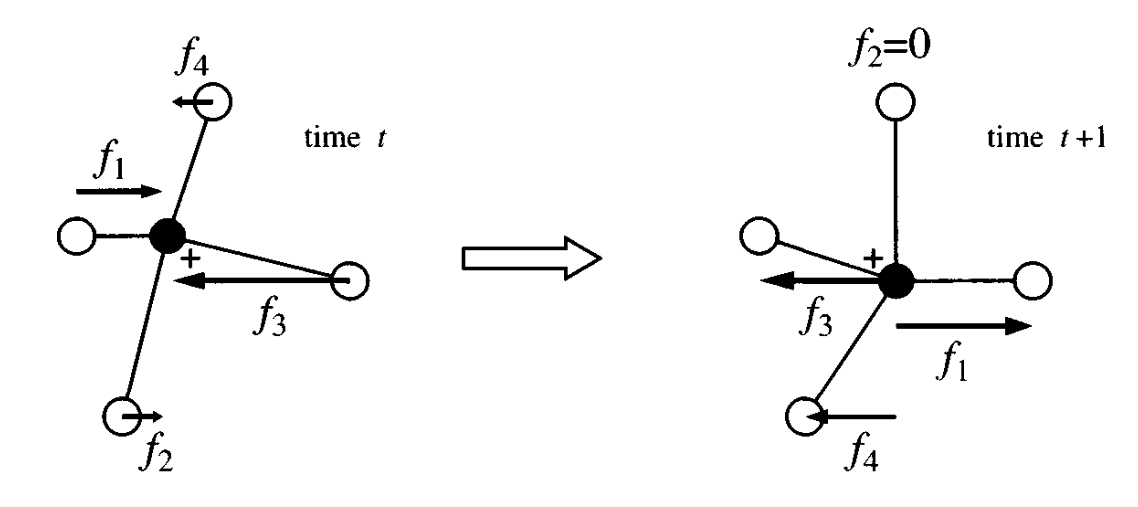
\includegraphics[width=0.7\textwidth]{Chopard_2D_cellular_automata.png}
%     \caption{Cellular automata scheme for 2D waves propagation.}
%     \label{fig:chopard_2D_waves_cellular_automata}
% \end{figure}

If the position of the black particle is $\vec r_{i,j} = (x_{i,j},y_{i,j})$ and the position of each white neighbor particle is $\vec r_{i-1,j}$, $\vec r_{i+1,j}$, $\vec r_{i,j-1}$ and $\vec r_{i,j+1}$ the distances between the black particle and the white ones are
\begin{subequations}\label{eq:f_i_chopard}
\begin{equation}
    f_1(i,j,t) = x_{i-1,j}(t) - x_{i,j}(t)
\end{equation}
\begin{equation}
    f_2(i,j,t) = x_{i,j-1}(t) - x_{i,j}(t)
\end{equation}
\begin{equation}
    f_3(i,j,t) = x_{i+1,j}(t) - x_{i,j}(t)
\end{equation}
\begin{equation}
    f_4(i,j,t) = x_{i,j+1}(t) - x_{i,j}(t)
\end{equation}
\end{subequations}
To deduct the evolution rule easier, we consider the case where the black particle is at the origin, that is $x_{i,j}(t) = 0$, then the x-coordinate of the mass center of the white particles is simply
\begin{equation}
    X_{CM} = \frac{1}{4}(f_1 + f_2 + f_3 + f_4)
\end{equation}


then the black particle will try to oscillate around the center of mass $X_{CM}$, thus it will reach a symmetrical position with respect to the center of mass. This leads to
\begin{equation}
    x_{i,j}(t+1) = 2 X_{CM} = \frac{1}{2}(f_1 + f_2 + f_3 + f_4)
\end{equation}
while the white particles will move at the next step, we need to compute the distances written in \ref{eq:f_i_chopard} but respect to the position of each white particle
\begin{align}
    f_1(i+1,j,t+1) &= x_{i,j}(t+1) - x_{i+1,j}(t+1) \\
    &= 2 X_{CM} - x_{i+1,j}(t+1)
\end{align}
so that using \ref{eq:f_i_chopard} we may write 
\begin{align}
    f_1(i+1,j,t) &= \frac{1}{2}(f_1 + f_2 + f_3 + f_4) - f_3 \\
    &= \frac{1}{2}(f_1 + f_2 - f_3 + f_4)
\end{align}

Following a similar procedure for $f_2$, $f_3$ and $f_4$ the evolution rule may be written in the following matrix representation
\begin{equation}\label{eq:evolution_rule_waves}
    \begin{pmatrix}
        f_1(i+1,j,t+1) \\
        f_2(i,j+1,t+1) \\
        f_3(i-1,j,t+1) \\
        f_4(i,j-1,t+1) \\        
    \end{pmatrix}
    =
    \bm{W}\begin{pmatrix}
        f_1(i,j,t) \\
        f_2(i,j,t) \\
        f_3(i,j,t) \\
        f_4(i,j,t) \\        
    \end{pmatrix}
\end{equation}
defining the matrix 
\begin{equation}\label{eq:W_chopard_evolution_rule}
    \bm{W} = \frac{1}{2}\begin{pmatrix}
        1 & 1 & -1 & 1 \\
        1 & 1 & 1 & -1 \\
        -1 & 1 & 1 & 1 \\
        1 & -1 & 1 & 1 \\
    \end{pmatrix}
\end{equation}
Chopard have shown that with this cellular automata is possible to simulate waves propagation in two dimensions. Then he shows how to obtain a similar evolution rule using the Lattice-Boltzmann equation \ref{eq:LBE_BGK}. 

In order to reproduce the evolution rule written in \ref{eq:evolution_rule_waves} using \ref{eq:LBE_BGK} we define the following macroscopic variables:
\begin{equation}\label{eq:chopard_fields}
    \Psi = \sum_i f_i \quad;\quad J_{\alpha} = \sum_i v_{i\alpha}f_i
\end{equation}
where this time the velocity set is still D2Q5 but they fulfil the next relationships:
\begin{subequations}
\begin{equation}
    \sum_{i=0}^4 v_{i\alpha} = 0
\end{equation}
\begin{equation}
    \sum_{i=0}^4 v_{i\alpha}v_{i\beta} = 2v^2\delta_{\alpha\beta}
\end{equation}
\end{subequations}
where $v$ is the magnitude of every velocity vector, for D2Q5 $v=1$.

Defining $a_0$ and $a$ which satisfy
\begin{equation}
    a_0 + 4a = 1
\end{equation} 
The equilibrium function is then
\begin{equation}\label{eq:chopard_feq}
    f_i^{\text{eq}} = \begin{cases}
        a_0\Psi & i=0\\
        a\Psi + \frac{\vec v_i \cdot \vec J}{2v^2} & i\neq0 
    \end{cases}
\end{equation}
Now, if we plug in \ref{eq:chopard_feq} into the Lattice-Boltzmann evolution rule with the BGK collision operator \ref{eq:LBE_BGK} we have for $i=0$
\begin{align}
    f_0(\vec x, t + \delta t) &= \frac{1}{\tau}\left( (\tau - 1)f_0 + a_0\Psi \right) \nonumber\\
    &= \frac{1}{\tau}\left((a_0+\tau-1)f_0 + a_0(f_1+f_2+f_3+f_4)\right)
\end{align}
and for $i\neq0$
\begin{equation}\label{eq:chopard_waves_evolution_rule_f0}
    f_i(\vec x+\delta t\vec v_i, t + \delta t) = \frac{1}{\tau}\left( a\Psi + \frac{\vec v_i \cdot \vec J}{2v^2} + (\tau-1)f_i \right)
\end{equation}

and after plugging in \ref{eq:chopard_fields} and doing some algebra 
\begin{align}\label{eq:chopard_waves_evolution_rule_fi}
    f_i(\vec x+\delta t\vec v_i, t + \delta t) &= \frac{1}{\tau}\bigg(\left(a+\tau-\frac{1}{2}\right)f_i+\dots\nonumber\\
    &\dots+ a f_{i+1} + \left(a-\frac{1}{2}\right)f_{i+2} + a f_{i+3} + a f_0\bigg)
\end{align}
This evolution rule defined in \ref{eq:chopard_waves_evolution_rule_f0} and \ref{eq:chopard_waves_evolution_rule_fi} may also be written as the following matrix equation
\begin{equation}
    \begin{pmatrix}
        f_0(\vec x, t + \delta t) \\
        f_1(\vec x+\delta t\vec v_i, t + \delta t) \\
        f_2(\vec x+\delta t\vec v_i, t + \delta t) \\
        f_3(\vec x+\delta t\vec v_i, t + \delta t) \\
        f_4(\vec x+\delta t\vec v_i, t + \delta t) \\        
    \end{pmatrix}
    =
    \bm{W'}\begin{pmatrix}
        f_0(\vec x, t) \\
        f_1(\vec x, t) \\
        f_2(\vec x, t) \\
        f_3(\vec x, t) \\
        f_4(\vec x, t) \\        
    \end{pmatrix}
\end{equation}

where the matrix $\bm{W'}$ is written as
\begin{equation}
    \bm{W'} = \frac{1}{\tau}\begin{pmatrix}
        a_0 + \tau - 1 & a_0 & a_0 & a_0 & a_0 \\
        a & a + \tau - 1/2 & a & a - 1/2 & a \\
        a & a & a + \tau - 1/2 & a & a - 1/2 \\
        a & a - 1/2 & a & a + \tau - 1/2 & a \\
        a & a & a - 1/2 & a & a + \tau - 1/2 \\
    \end{pmatrix}
\end{equation}
the interesting about $\bm{W'}$ is that for $i\neq0$ and $a_0 = 0$ we get
\begin{equation}
    \bm{W'} = \frac{1}{\tau}\begin{pmatrix}
        \tau - 1 & 0 & 0 & 0 & 0 \\
        1/4 & \tau - 1/4 & 1/4 & -1/4 & 1/4 \\
        1/4 & 1/4 & \tau - 1/4 & 1/4 & -1/4 \\
        1/4 & -1/4 & 1/4 & \tau - 1/4 & 1/4 \\
        1/4 & 1/4 & -1/4 & 1/4 & \tau - 1/4 \\
    \end{pmatrix}
\end{equation}

Finally, if we chose $\tau=1/2$ the resulting matrix will be
\begin{equation}
    \bm{W'} = \frac{1}{2}\begin{pmatrix}
        -2 & 0 & 0 & 0 & 0 \\
        1 & 1 & 1 & -1 & 1 \\
        1 & 1 & 1 & 1 & -1 \\
        1 & -1 & 1 & 1 & 1 \\
        1 & 1 & -1 & 1 & 1 \\
    \end{pmatrix}
\end{equation}
which is similar to the matrix $\bm{W}$ written in equation \ref{eq:W_chopard_evolution_rule}. The LB model shown here solves the equations
\begin{subequations}
\begin{equation}
    \partial_t \Psi + \partial_\alpha J_\alpha = 0
\end{equation}
\begin{equation}
    \partial_t J_\alpha + \partial_\beta\Pi_{\alpha\beta} = 0
\end{equation}
\end{subequations}
where
\begin{equation}
    \Pi_{\alpha\beta} = 2av^2\Psi\delta_{\alpha\beta}
\end{equation}
matching also \ref{eq:escalar_continuity} and \ref{eq:vector_continuity} if $\tau=1/2$. 

The waves equation is easily obtained using a similar procedure as in \ref{eq:proc_waves_rho} or \ref{eq:proc_waves_p} getting
\begin{equation}
    \partial_t^2\Psi = 2av^2\nabla^2\Psi
\end{equation}
where the propagation speed is identified as $c\equiv v\sqrt{2a}$ which depends on the free parameter $a$. This lets to adjust the speed making possible to model various refraction indexes and describing inhomogeneous media. 
% \begin{figure}
%     \centering
%     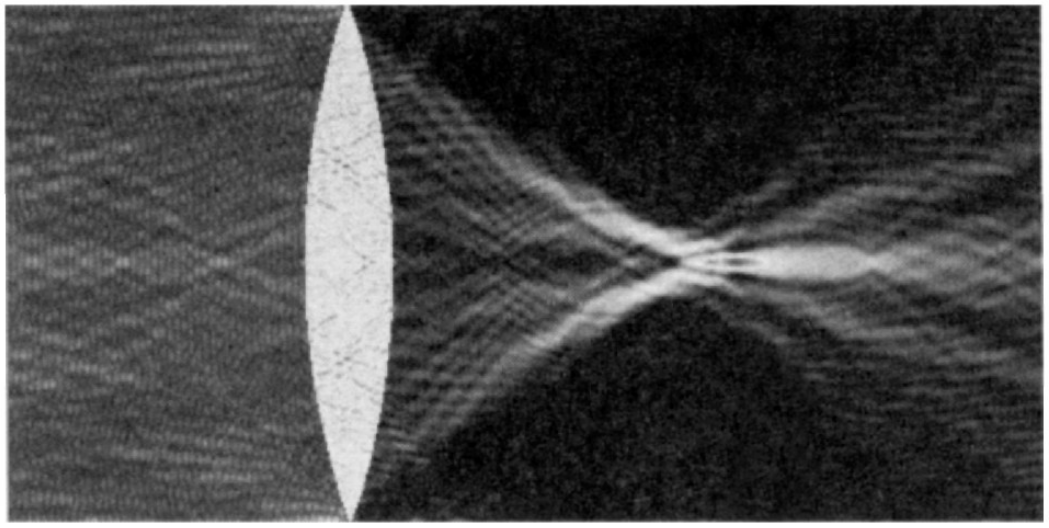
\includegraphics[width=0.4\textwidth]{lens_LB_chopard.png}
%     %\caption{Caption}
%     \label{fig:lens}
% \end{figure}
The Chopard's model solves the waves equation for a \textbf{generic scalar field} $\Psi$ with the help of an \textbf{auxiliary generic vector field} $\vec J$ regardless their physical meaning. \textit{However, if we want to adjust the speed we need to be careful of possible dependencies of $c$ in any of the fields.} 

As we have neglected the non-linear term $\rho u_{\alpha1}u_{\beta1}$ the momentum flux density tensor $\Pi_{\alpha\beta}$ has become the \textbf{diagonal} tensor
\begin{equation}
    \Pi_{\alpha\beta} = p_1\delta_{\alpha\beta} = c_s^2\rho_1\delta_{\alpha\beta}
\end{equation}
Therefor, if we want to use the Lattice-Boltzmann method to simulate the waves we shall use instead the following macroscopic variables
\begin{equation}
    \rho_1 = \sum_i f_i \quad;\quad \rho_0 u_{\alpha1} = \sum_i v_{i\alpha}f_i  \quad;\quad \Pi_{\alpha\beta} = p_1\delta_{\alpha\beta} = \sum_i v_{i\alpha}v_{i\beta}f_i
\end{equation}
and the equilibrium function that produces these macroscopic quantities is simply
\begin{equation}\label{eq:eq_function_waves_from_fluids}
    f_i^{\text{eq}} = \rho_1\omega_i + \rho_0\omega_i\frac{v_{i\alpha}u_{\alpha1}}{c_s^2}
\end{equation}
coinciding with the equilibrium function for fluids without the quadratic terms of velocity. 

The issue with this model is that $c_s^2$ comes from the conditions defined in \ref{eqs:sums_vw} which involve the velocities and weights set. If we want to change $c_s^2$ we need then to modify the weights such that \ref{eqs:sums_vw} still hold. Taking a lattice as D2Q5, \textbf{where only the first four equations of \ref{eqs:sums_vw} are satisfied}, we have:
\begin{equation}
    \{\vec v_i\} = \left\{\begin{bmatrix}
        0 \\
        0
    \end{bmatrix};\begin{bmatrix}
        1 \\
        0
    \end{bmatrix};\begin{bmatrix}
        0 \\
        1
    \end{bmatrix};\begin{bmatrix}
        -1 \\
        0
    \end{bmatrix};\begin{bmatrix}
        0 \\
        -1
    \end{bmatrix}\right\}
\end{equation}
and the weights are determined by \ref{eqs:sums_vw}, such that for \ref{eq:sum_wi} we have
\begin{equation}\label{eq:weights_first}
    \sum_i \omega_i = \omega_0 + \omega_1 + \omega_2 + \omega_3 + \omega_4 = 1
\end{equation}
for equation \ref{eq:sum_viwi},
\begin{align}
    \sum_i v_{x}\omega_i = \omega_1 - \omega_3 = 0\quad&\text{and}\quad\sum_i v_{y}\omega_i = \omega_2 - \omega_4 = 0 \nonumber\\
    \omega_1 = \omega_3\quad&\text{and}\quad\omega_2 = \omega_4 \label{eq:weights_second}
\end{align}

and for equation \ref{eq:sum_viviwi} 
\begin{align}
    \sum_i v_{x}v_{x}\omega_i = \omega_1 + \omega_3 = c_s^2\quad&\text{and}\quad\sum_i v_{y}v_{y}\omega_i = \omega_2 + \omega_4 = c_s^2 \nonumber\\
    \omega_1 = \frac{c_s^2}{2}\quad&\text{and}\quad\omega_2 = \frac{c_s^2}{2} \nonumber\\
    \sum_i v_{x}v_{y}\omega_i = 0 \quad&\text{and}\quad\sum_i v_{y}v_{x}\omega_i = 0 \label{eq:weights_third}
\end{align}
And replacing \ref{eq:weights_second} and \ref{eq:weights_third} into \ref{eq:weights_first} we end up with $i\neq0$
\begin{align}
    \omega_i &= \frac{c_s^2}{2} \label{eq:weight0_solution}\\
    \omega_0 &= 1 - 4\omega_i = 1 - 2c_s^2\label{eq:weights_solution}
\end{align}
which is consistent with the case $c_s = 1/\sqrt{3}$, $\omega_0 = 1/3$ and $\omega_i = 1/6$. Note that this only works for D2Q5.

Using this results the equilibrium function written in \ref{eq:eq_function_waves_from_fluids} will take the form
\begin{equation}
    f_i^{\text{eq}} = \begin{cases}
        (1 - 2 c_s^2)\rho_1 = \omega_0\rho_1 & i=0 \\
        \frac{c_s^2}{2}\rho_1 + \frac{v_{i\alpha}(\rho_0 u_\alpha)}{2} = \omega_i\rho_1 + \frac{v_{i\alpha}(\rho_0 u_\alpha)}{2} & i\neq0 \\
    \end{cases} 
\end{equation}
now from \ref{eq:weight0_solution} and \ref{eq:weights_solution} of the D2Q5 lattice, equation \ref{eqs:sums_vw} becomes simply
\begin{subequations}\label{eqs:sums_vw}
\begin{equation}\label{eq:sum_wi_waves}
    \omega_0 + 4\omega_i = 1
\end{equation}
\begin{equation}\label{eq:sum_viwi_waves}
    \sum_i v_{i\alpha}\left(\frac{c_s^2}{2}\right) = 0
\end{equation}
\begin{equation}\label{eq:sum_viviwi_waves}
    \sum_i v_{i\alpha}v_{i\beta}\left(\frac{c_s^2}{2}\right) = c_s^2\delta_{\alpha\beta}
\end{equation}
\begin{equation}\label{eq:sum_viviviwi_waves}
    \sum_i v_{i\alpha}v_{i\beta}v_{i\gamma}\left(\frac{c_s^2}{2}\right) = 0
\end{equation}
\end{subequations}

Notice that \ref{eq:sum_viwi_waves} and \ref{eq:sum_viviwi_waves} become
\begin{subequations}
\begin{equation}\label{eq:sum_viwi_waves}
    \sum_i v_{i\alpha}= 0
\end{equation}
\begin{equation}\label{eq:sum_viviwi_waves}
    \sum_i v_{i\alpha}v_{i\beta} = 2\delta_{\alpha\beta}
\end{equation}
\end{subequations}
Such that once 
